\begin{figure}[hbtp]
\includegraphics[width=\columnwidth]{distag}
\caption{Tag distribution log-log scale over three regions of different scale.\label{f:tags}}
\end{figure}

The first thing was to look at the tags to get a sense of them. In San
Francisco after the preprocessing, there was a total of \numprint{4977625}
occurrences of the \numprint{145242} unique tags. But their distribution varies
widely, between the most popular one, \textsf{sanfrancisco}, used
\numprint{373427} times and the \numprint{101361} that are used less than 5
times. Some of them are shown in Table~\vref{tab:tags} but a more synthetic
visualization is presented in Figure~\vref{f:tags}, where we can see that like
words in a written documents, tags follows a power law.

\begin{table}[ht]
	\centering
	\begin{tabular}{lll}
		\toprule
		First 15 tags 	 & between 100 and 1000 & after \numprint{90000} \\
		\midrule
		sanfrancisco 	 & 2013 							   & sfgiantsfan \\
		california       & pacific                             & rolexbigboatseries \\
		iphoneography    & february                            & proshowgold \\
		square           & foundinsf                           & neutraface \\
		% squareformat     & dolorespark                         & natur€ \\
		instagramapp     & japaneseteagarden                   & lusty \\
		unitedstates     & boat                                & lightousetender \\
		sf               & 5k                                  & jennyholzer \\
		usa              & national                            & img0562jpg \\
		% ca               & σανφρανσίσκο                        & djguyruben \\
		san              & cruise                              & cutebaby \\
		francisco        & above                               & cardamine \\
		goldengatepark   & july2009                            & californiaproduce \\
		2010             & effortlesslyuploadedbymyeyeficard   & aroundwithb1 \\
		iphone           & dayofdecision                       & aquateenhungerforcemooninite \\
		\bottomrule
	\end{tabular}
	\caption{A sample of San Francisco tags, depending of their rank.\label{tab:tags}}
\end{table}

After making these observations, I decided to consider only tags with enough
support, both to ease the computational effort and to avoid outliers. For each
tags, I compute three simple metrics, total count, distinct users count and
time span. Using the three threshold (150 photos, 25 users, 500 days), I kept
only \numprint{1836} tags. It may seem quite restrictive but they still cover
68.6\% of all occurrences and we can always change these thresholds
later\footnote{For instance, with $(20, 2, 0)$, we get \numprint{12959} tags
and 84.4\% coverage.}.

We can then conduct a similar analysis over the locations in which photos
appear. Because of their large number, it was not convenient nor readable to
display them individually. Therefore, I discretized space as a regular grid of
size 200 by 200. In that case, each rectangular cell is around $80\times 70$
meters and I used this same method for all other spatial computation. A
natural way of visualizing them is to draw a heatmap (Figure~\vref{f:heat}).
We notice again that they are far from being uniformly distributed and that
some neighborhood are more popular than others. More quantitatively, number of
photos of each location as a function of their rank (Figure~\vref{f:pdis}), we
notice that it first follows a power law and after some point, a more
abrupt one. Moreover, the same phenomena occurs for other grid size, albeit
with different $\alpha$ coefficient. Despite this similar behavior, it was
more tricky to explicitly exclude parts of the city.

\begin{figure}[hbtp]
\includegraphics[width=\columnwidth]{../heatmap.png}
\caption{Photos count in logarithmic scale (the darker, the more
photos).\label{f:heat}}
\end{figure}

\begin{figure}[hbtp]
\includegraphics[width=\columnwidth]{../prez/pdistrib.png}
\caption{Spatial distribution of photos over three grids with different
granularity.\label{f:pdis}}
\end{figure}

Let us return to one of our original problem, find which tags describe a given
location. The first approach would to filter this \numprint{1836} tags to keep
only those that are enough concentrated at one position and reject those that
too uniformily distributed. After that, it would simply a matter of returning
those that appear in the place of interest. An example of this two kind of
tags are \textsf{museum} and \textsf{street}. As shown in Figure~\vref{f:sm},
\textsf{museum} photos are mostly located around five or six points whereas
\textsf{street} is more diffuse. But instead of looking at a map, we want a
numerical statistic that allow us to distinguish between this two cases.

\begin{figure}[hbtp]
\includegraphics[width=\columnwidth]{../prez/sm.png}
\caption{Red dots denote photos tagged \textsf{museum} while blue ones are
	\textsf{street}.\label{f:sm}}
\end{figure}

\begin{wrapfigure}[5]{r}{0.2\textwidth}
\centering
\vspace{-.6\baselineskip}
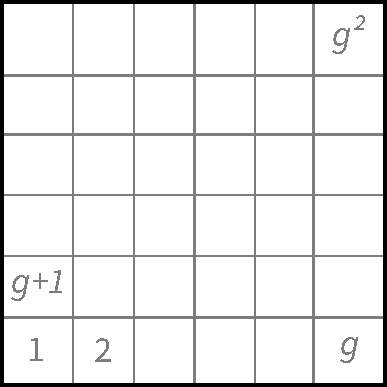
\includegraphics[width=0.15\columnwidth]{grid}
\end{wrapfigure}
Let first define some notation. As mentioned before, the city is divided in a
$g\times g$ grid made of rectangular cells $1$ through $g^2$ (like pictured on
the right).  For a cell $i$, let $b(i)$ be the total number of photos in cell
$i$\footnote{The so called background, hence the notation.}, $B=\sum_i b(i)$
the total number of photos and $b_f(i)$ the frequency of each cell. For a tag
$t$, we define in the same manner, $t(i)$, $T$ and $t_f(i)$, this time
considering only photos which have tags $t$.

With these frequencies we can compute entropy. Let $H(t,g) = -\frac{1}{2\log
g}\sum_{i=1}^{g^2} t_f(i)\log t_f(i)$ be the entropy of tag $t$ on a grid of
size $g$. The normalization factor ensure that regardless of $g$, the values
will range from 0 (all photos in the same cell) to 1 (uniform distribution).

\begin{table}[ht]
\centering
\begin{tabular}{lclclc}
\toprule
 \multicolumn{2}{c}{$g=200$}&  \multicolumn{2}{c}{$g=80$}&  \multicolumn{2}{c}{$g=20$}  \\
\midrule
\multicolumn{6}{c}{Lowest entropy} \\
\midrule
111minna         & .046 & theindependent         & .008 & museumofmodernart   & .002 \\
billgraham[…]    & .052 & dnalounge              & .012 & yerbabuena[…]       & .003 \\
rodin            & .053 & franklloydwright       & .022 & californiapalace[…] & .003 \\
teagarden        & .058 & greatamericanmusichall & .022 & museemecanique      & .006 \\
dnalounge        & .063 & californiapalace[…]    & .025 & cupidsspan          & .007 \\
bottomofthehill  & .064 & bottomofthehill        & .025 & pier45              & .007 \\
cafedunord       & .067 & saintspeter[…]         & .026 & missiondolorespark  & .008 \\
theindependent   & .069 & rodin                  & .034 & theindependent      & .010 \\
franklloydwright & .070 & honor                  & .035 & clarionalley        & .011 \\
warfield         & .074 & billgraham[…]          & .035 & asianartmuseum      & .012 \\
greatamerican[…] & .075 & asianartmuseum         & .038 & fairmont            & .012 \\
\midrule
\multicolumn{6}{c}{Highest entropy} \\
\midrule
usa              & .688 & color                  & .728 & sunset              & .751 \\
sf               & .696 & northerncalifornia     & .729 & dog                 & .753 \\
instagramapp     & .700 & square                 & .735 & purple              & .755 \\
square           & .700 & instagramapp           & .736 & nikon               & .756 \\
squareformat     & .700 & squareformat           & .736 & sky                 & .757 \\
iphoneography    & .703 & iphoneography          & .737 & blue                & .766 \\
unitedstates     & .703 & iphone                 & .737 & d200                & .767 \\
iphone           & .720 & california             & .738 & color               & .769 \\
foundinsf        & .724 & sanfrancisco           & .744 & northerncalifornia  & .773 \\
california       & .726 & gwsf                   & .766 & gwsf                & .812 \\
sanfrancisco     & .738 & foundinsf              & .803 & foundinsf           & .825 \\
\bottomrule
\end{tabular}
\caption{long (the abbreviated tags are \textsf{billgrahamcivicauditorium},
	\textsf{californiapalaceofthelegionofhonor},
	\textsf{yerbabuenacenterforthearts}, \textsf{greatamericanmusichall} and
\textsf{saintspeterandpaulchurch}).\label{tab:entropy}}
\end{table}
